\documentclass[margin=0mm]{standalone}
\usepackage{tikz}
\usepackage{pgfplots}
 \pgfplotsset{compat=newest}

\usepgfplotslibrary{fillbetween}

\usetikzlibrary{calc}

\begin{document}


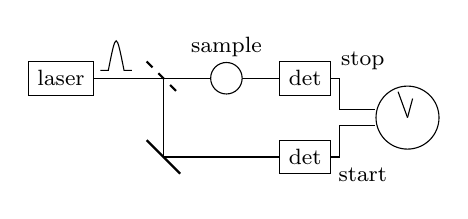
\begin{tikzpicture}[font=\footnotesize]
%\useasboundingbox (0,0) rectangle (5,5);
%\draw (0,0) rectangle (5,5);


\coordinate (laser) at (0,0);
\coordinate (bs1) at ($(laser) + (1.3,0)$);
\coordinate (m1) at ($(bs1) + (0,-1)$);
\coordinate (sample) at ($(bs1) + (0.8,0)$);
\coordinate (det1) at ($(sample) + (1,0)$);
\coordinate (det2) at ($(det1) + (0,-1)$);
\coordinate (clock) at ($(det1) + (1.3,-0.5)$);



\draw (laser.west) -- (det1.east);
\draw (bs1) -- (m1) -- (det2.east);

\draw (0.5, 0.1) -- (0.6, 0.1) .. controls (0.7, 0.6) .. (0.8,0.1) --(0.9,0.1);

\node[rectangle, draw, fill=white] at (laser) {laser} ;
\draw [dashed, thick] ($(bs1) + (135:3mm)$) -- ++(-45:6mm) ;

\draw [fill=white] (sample) circle (2mm);
%\draw [dashed, thick] ($(bs2) + (45:3mm)$) -- ++(-135:6mm) ;

\node (d1) [rectangle, draw, fill=white]  at (det1) {det} ;
\node (d2) [rectangle, draw, fill=white]  at (det2) {det} ;

\draw [solid, thick] ($(m1) + (135:3mm)$) -- ++(-45:6mm) ;
\node (c) [circle, draw, fill=white, minimum width=8mm]  at (clock) {};

\draw (d1.east) |- +(1mm,0) |-  ($ (c.west) + (0,1mm)$);
\draw (d2.east) |- +(1mm,0) |-  ($ (c.west) + (0,-1mm)$);

\draw (clock) -- ++ (110:3.5mm);
\draw (clock) -- ++ (75:2.5mm);

\node at (sample) [yshift=+4mm] {sample};
\node at (d1.north east) [xshift=+4mm] {stop};
\node at (d2.south east) [xshift=+4mm] {start};


%\draw [solid, thick] ($(m2) + (45:3mm)$) -- ++(-135:6mm) ;
%
%\node at (lamp) [yshift=-4mm, xshift=2mm] {lamp};

%\node at (ref) [yshift=-4mm] {reference};
%\node at (bs1) [yshift=4mm, xshift=-7mm]{flip mirror};

\end{tikzpicture}


\end{document}